\documentclass[12pt,a4paper]{article}

% --- 1. Khai báo các gói tiếng Việt và căn lề ---
\usepackage[utf8]{vietnam}
\usepackage[top=2cm, bottom=2cm, left=2cm, right=2cm]{geometry}
\usepackage{graphicx}
\usepackage{float}

% --- 2. Gói bắt buộc để tạo bảng longtable và tô màu ---
\usepackage{longtable}
\usepackage[table]{xcolor}

% --- 3. Định nghĩa màu xanh nhạt tiêu đề bảng ---
\definecolor{tableheader}{RGB}{211, 228, 205}

\begin{document}
	

	% --- CHÈN SƠ ĐỒ ---
	\vspace*{\fill}
	\begin{figure}[H]
		\centering
		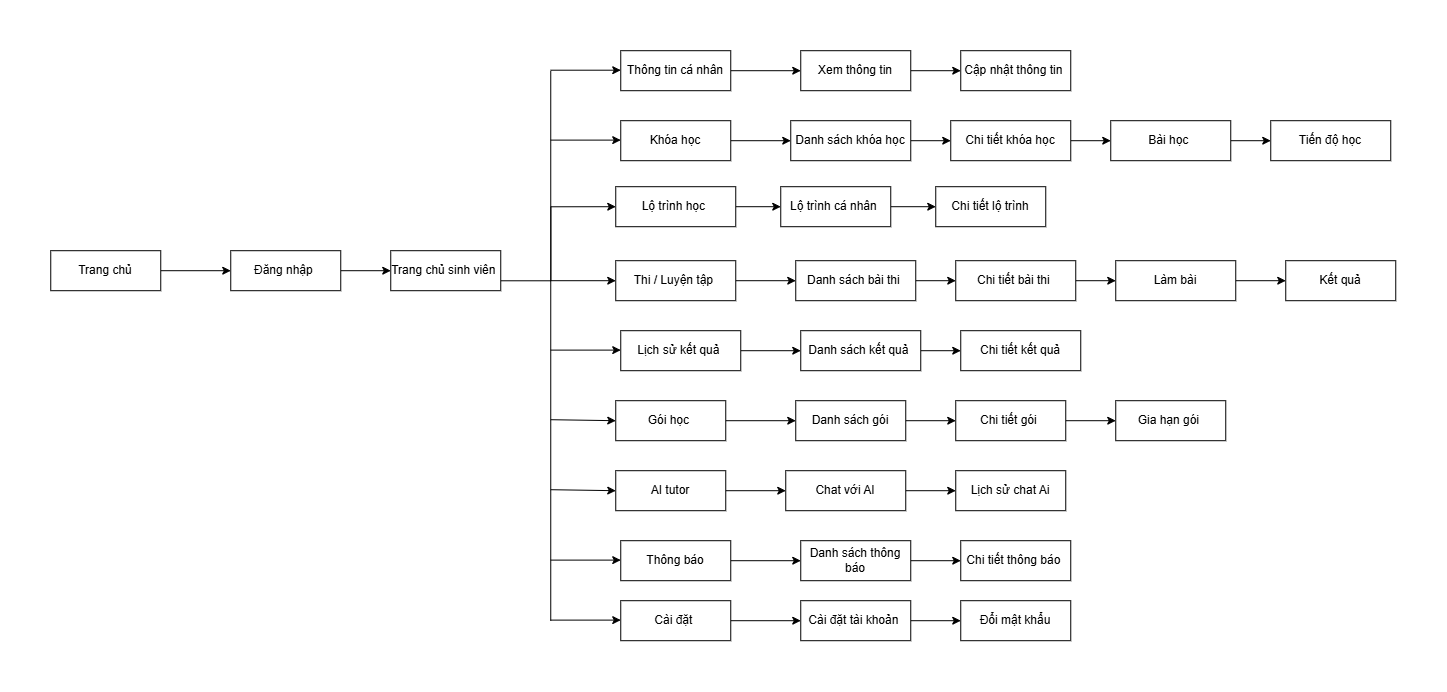
\includegraphics[width=\textwidth]{Figure/screenflow-trang1.drawio.png}
		\caption{Sơ đồ luồng màn hình Sinh Viên}
		\label{fig:screenflow}
	\end{figure}
	\vfill
	
	\clearpage
	
	\section{Screenflow Descriptions}
	
	\begin{longtable}{|p{3.2cm}|p{5.5cm}|p{7.3cm}|}
		\hline
		\rowcolor{tableheader}
		\textbf{Feature} & \textbf{Screen} & \textbf{Description} \\ \hline
		\endhead
		
		General & Trang chủ / Đăng nhập / Trang chủ sinh viên & Màn hình khởi đầu và đăng nhập tài khoản dành cho sinh viên để truy cập vào hệ thống. \\ \hline
		
		Profile & Thông tin cá nhân / Xem thông tin / Cập nhật thông tin & Cho phép sinh viên xem chi tiết hồ sơ cá nhân và chỉnh sửa, cập nhật thông tin tài khoản. \\ \hline
		
		Course & Khóa học / Danh sách khóa học / Chi tiết khóa học / Bài học / Tiến độ học & Quản lý danh sách khóa học đăng ký, truy cập nội dung bài học và theo dõi tiến độ hoàn thành. \\ \hline
		
		Learning Path & Lộ trình học / Lộ trình cá nhân / Chi tiết lộ trình & Định hướng và hiển thị chi tiết các bước trong lộ trình học tập cá nhân hóa của sinh viên. \\ \hline
		
		Examination & Thi - Luyện tập / Danh sách bài thi / Chi tiết bài thi / Làm bài / Kết quả & Cho phép sinh viên chọn bài thi, thực hiện bài làm trực tuyến và xem kết quả đánh giá ngay. \\ \hline
		
		Result History & Lịch sử kết quả / Danh sách kết quả / Chi tiết kết quả & Bảng tổng hợp lịch sử điểm số và chi tiết bài làm của các kỳ thi/luyện tập đã hoàn thành. \\ \hline
		
		Subscription & Gói học / Danh sách gói / Chi tiết gói / Gia hạn gói & Quản lý thông tin các gói dịch vụ học tập, xem ưu đãi và thực hiện đăng ký hoặc gia hạn gói. \\ \hline
		
		AI Tutor & AI tutor / Chat với AI / Lịch sử chat AI & Trợ lý ảo AI hỗ trợ giải đáp thắc mắc học tập, tương tác trực tiếp và lưu lại lịch sử hội thoại. \\ \hline
		
		Notification & Thông báo / Danh sách thông báo / Chi tiết thông báo & Cập nhật danh sách các thông báo mới từ hệ thống, tin tức khóa học và nhắc nhở lịch thi. \\ \hline
		
		Settings & Cài đặt / Cài đặt tài khoản / Đổi mật khẩu & Cho phép sinh viên thiết lập cấu hình tài khoản cá nhân và thực hiện thay đổi mật khẩu. \\ \hline
		
	\end{longtable}
	
	\vspace*{\fill}
	\begin{figure}[H]
		\centering
		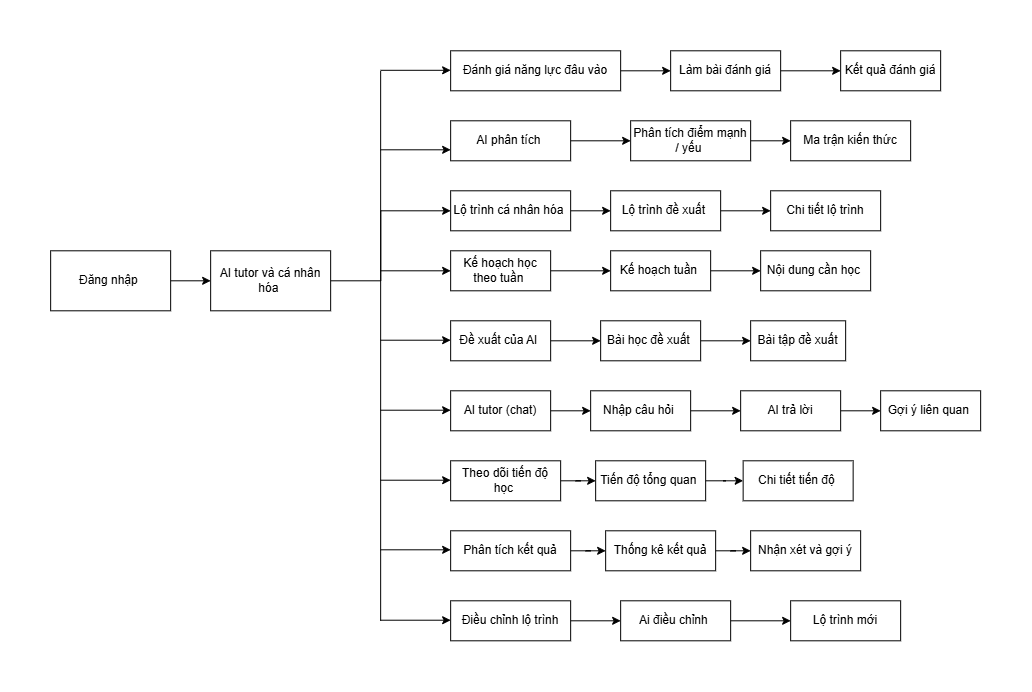
\includegraphics[width=\textwidth]{Figure/screenflow-trang2.drawio.png}
		\caption{Sơ đồ luồng màn hình AI Tutor Và Cá Nhân Hóa Lộ Trình}
		\label{fig:screenflow}
	\end{figure}
	\vfill
	
	\clearpage
	
	\begin{longtable}{|p{3.2cm}|p{5.5cm}|p{7.3cm}|}
		\hline
		\rowcolor{tableheader}
		\textbf{Feature} & \textbf{Screen} & \textbf{Description} \\ \hline
		\endhead
		
		Initial Assessment & Đánh giá năng lực đầu vào / Làm bài đánh giá / Kết quả đánh giá & Cho phép sinh viên thực hiện bài kiểm tra đầu vào để xác định trình độ và nhận đánh giá năng lực ban đầu. \\ \hline
		
		AI Analysis & AI phân tích / Phân tích điểm mạnh - yếu / Ma trận kiến thức & Hệ thống AI phân tích chi tiết các điểm mạnh, điểm yếu và lập ma trận kiến thức cho sinh viên. \\ \hline
		
		Personalized Path & Lộ trình cá nhân hóa / Lộ trình đề xuất / Chi tiết lộ trình & Hiển thị các bước trong lộ trình học tập được thiết kế riêng dựa trên năng lực cá nhân. \\ \hline
		
		Weekly Plan & Kế hoạch học theo tuần / Kế hoạch tuần / Nội dung cần học & Phân bổ mục tiêu học tập và danh sách nội dung bài học cụ thể cần hoàn thành trong từng tuần. \\ \hline
		
		AI Recommendation & Đề xuất của AI / Bài học đề xuất / Bài tập đề xuất & Gợi ý tự động các bài học và bài tập luyện tập bổ trợ tối ưu nhất do AI phân tích. \\ \hline
		
		AI Chatbot & AI tutor (chat) / Nhập câu hỏi / AI trả lời / Gợi ý liên quan & Giao diện trò chuyện trực tiếp với trợ lý AI, nhận câu trả lời và các gợi ý chủ đề liên quan. \\ \hline
		
		Progress Tracking & Theo dõi tiến độ học / Tiến độ tổng quan / Chi tiết tiến độ & Cung cấp báo cáo tổng quan và số liệu chi tiết về mức độ hoàn thành bài học. \\ \hline
		
		Result Analysis & Phân tích kết quả / Thống kê kết quả / Nhận xét và gợi ý & Thống kê chi tiết kết quả học tập kèm các nhận xét và gợi ý cải thiện từ hệ thống. \\ \hline
		
		Path Adjustment & Điều chỉnh lộ trình / AI điều chỉnh / Lộ trình mới & AI tự động cập nhật và điều chỉnh lại lộ trình học tập mới phù hợp với sự tiến bộ của sinh viên. \\ \hline
		
	\end{longtable}
	
	
\end{document}